\chapter{OLFACTION SENSING BASED ROSL ALGORITHM}\label{chap:olfaction}

\section{Introduction}
% background and problem statement
Many prior works (see ~\ref{Subsec:olfactionRelatedResearch}) only validated ROSL algorithms in simulation environments. However, simulation environments cannot always represent real-world scenarios due to the gap between simulation and real-world environments. 
This chapter discusses the development of a multi-modal robotic platform for real-world ROSL research and the implementation and evaluation of a traditional ROSL algorithm. The works covered in this chapter were published as a conference paper \cite{hassan2023multi}.

\subsection{Related Research}\label{Subsec:olfactionRelatedResearch}
% bio-inspired OSL
Designing algorithms that replicate the navigation methods of biological organisms is a common approach in robotic odor source localization research. Various organisms, regardless of their size, rely on scent to locate objects. Whether it is a bacterium navigating an amino acid gradient or a wolf tracking prey, the ability to follow odors is vital for survival.

Chemotaxis represents the simplest odor source localization strategy in biological organisms, where navigation relies solely on olfaction. For instance, bacteria demonstrate chemotaxis by altering their movement in response to changes in chemical concentration. When they encounter higher levels of an attractive chemical, their likelihood of making temporary turns decreases, resulting in straighter movement. Conversely, in the absence of a gradient or when moving away from higher concentrations, their default turning probability remains the same \cite{berg2000motile}. This straightforward algorithm allows single-celled organisms to navigate a gradient of appealing chemicals through a guided random walk. Nematodes \cite{lockery2011computational} and crustaceans \cite{radvansky2018olfactory} also utilize chemotaxis-based odor source localization. Early ROSL efforts focused on implementing such simple gradient-following chemotaxis algorithms. Typically, these methods used a pair of chemical sensors on plume-tracing robots, guiding them towards areas with higher concentration readings \cite{sandini1993gradient}. Several early studies \cite{grasso2000biomimetic, russell2003comparison, lilienthal2004experimental, ishida2005controlling} confirmed the effectiveness of chemotaxis in laminar flow environments, characterized by low Reynolds numbers. However, in turbulent flow environments with high Reynolds numbers, alternative methods inspired by more complex biological navigation techniques and engineering techniques were proposed.

Odor-gated anemotaxis navigation is a more sophisticated olfaction-based odor source localization method that uses both odor and airflow senses for navigation. Moths \cite{murlis1992odor, vickers2000mechanisms, carde2008navigational}, birds \cite{nevitt2000olfactory, wallraff2004avian}, and other organisms utilize this type of navigation. Specifically, mimicking the mate-seeking behavior of male moths led to the development of the moth-inspired method in ROSL research. This method has been successfully applied in various robotic OSL scenarios \cite{shigaki2017time}. Additionally, diverse bio-inspired search strategies such as zigzag, spiral, fuzzy-inference, and multi-phase exploratory approaches have been introduced in recent time\cite{shigaki2019modeling}. Recent bio-inspired OSL navigation methods have also aimed to increase the complexity of the search environment. For example, chemical plume tracking is performed in three-dimensional environments using three-dimensional moth-inspired OSL search \cite{rahbar20173, shigaki2022palm}.

Engineering-based methods differ from bio-mimicking algorithms by relying on mathematical models to estimate odor source locations. These approaches are often referred to as infotaxis \cite{vergassola2007infotaxis}. They involve constructing source probability maps, dividing the search area into regions, and assigning probabilities that indicate the likelihood of each region containing the odor source. Algorithms used for constructing such maps include Bayesian inference, particle filters, stochastic mapping \cite{jakuba2007stochastic}, source term estimation \cite{rahbar2019algorithm}, information-based search \cite{hutchinson2018information}, partially observable Markov decision processes \cite{hai2019underwater}, and combinations of infotaxis and the Dijkstra algorithm \cite{luong2023odor}. After predicting the odor source location, robots are then guided towards the estimated source via path-planning algorithms such as artificial potential fields and A-star \cite{pang2009reactive, wang2019chemical}.

\subsection{Objectives}\label{Subsec:mothObjectives}
The project has two main objectives:
\begin{itemize}
    \item to discuss the development of a versatile robotics platform - including robot hardware and software setup.
    \item to implement a traditional ROSL algorithm that can lead the mobile robot to the odor source in a real-world environment.
\end{itemize}


\section{Methodology}
\subsection{Hardware Setup}\label{Subec:OSLHardware}

\begin{figure}[h] %% figure

\ \\
\vspace*{-.18in}

\begin{center}
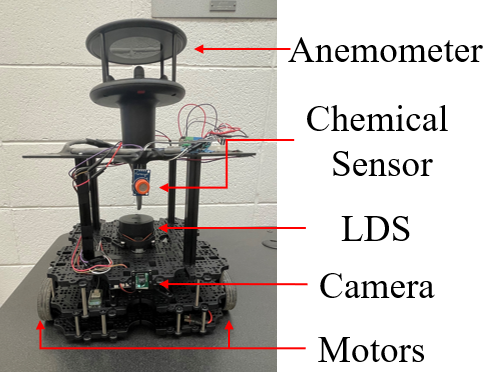
\includegraphics[width=0.6\columnwidth]{Main/Figure/olfaction_Turtlebot.png}\hspace*{0.04in}
\end{center}
\vspace{-.1in}

\caption
{The robot platform used in this work. In addition to the onboard sensors in Turtlebot3 model, the robot is equipped with a chemical sensor and an anemometer for measuring chemical concentration, wind speeds and directions.}
%\end{singlespace}
\label{fig:olfaction_robot}
\end{figure}

The Turtlebot3 mobile robot platform was utilized in this work. It comes equipped with a built-in camera, a LiDAR sensor, and a DYNAMIXEL driver for navigation. It is powered by Raspberry Pi 4. It uses Ubuntu and Robot Operating System (ROS) as operating systems. The onboard OpenCR controller enables the Turtlebot3 to be paired with additional sensors to enhance its functionality. Table~\ref{tab:sensors} lists the built-in and additional sensors used for OSL experiments. The Raspberry Pi Camera V2 was used for image capture, the LDS-02 Laser Distance Sensor for obstacle detection, the WindSonic Anemometer for measuring wind speed and direction in the body frame, and the MQ3 alcohol detector for detecting chemical plume concentration. Figure~\ref{fig:olfaction_robot} shows the final developed robotic platform.

\begin{table}[h]

\ \\

\caption{Type, name, and specification of the built-in camera, laser distance sensor, and added anemometer and chemical sensor.}
\label{tab:sensors}
\ \\
\centerline{
\begin{tabular}{|c|c|c|c|}
\hline
\textbf{Source}           & \textbf{Sensor Type}                                              & \textbf{Module Name}                                             & \textbf{Specification}                                                                                       \\ \hline
\multirow{2}{*}{Built-in} & Camera                                                            & \begin{tabular}[c]{@{}c@{}}Raspberry\\ Pi Camera v2\end{tabular} & \begin{tabular}[c]{@{}c@{}}Video Capture:\\ 1080p30, \\ 720p60 and VGA90.\end{tabular}                       \\ \cline{2-4} 
                          & \begin{tabular}[c]{@{}c@{}}Laser\\ Distance\\ Sensor\end{tabular} & LDS-02                                                           & \begin{tabular}[c]{@{}c@{}}Detection Range:\\ 360-degree.\\ Distance Range:\\ 160$\sim$8000 mm.\end{tabular} \\ \hline
\multirow{2}{*}{Added}    & Anemometer                                                        & \begin{tabular}[c]{@{}c@{}}WindSonic,\\ Gill Inc.\end{tabular}   & \begin{tabular}[c]{@{}c@{}}Speed:\\ 0--75 m/s.\\ Wind direction:\\ 0--360 degrees.\end{tabular}              \\ \cline{2-4} 
                          & \begin{tabular}[c]{@{}c@{}}Chemical\\ Sensor\end{tabular}         & \begin{tabular}[c]{@{}c@{}}MQ3 alcohol\\ detector\end{tabular}   & \begin{tabular}[c]{@{}c@{}}Concentration:\\ 25--500 ppm.\end{tabular}                                        \\ \hline
\end{tabular}

}

\ \\
\vspace{-.1in}

\end{table}

\begin{figure}[h]

\ \\
\vspace*{-.18in}

\begin{center}
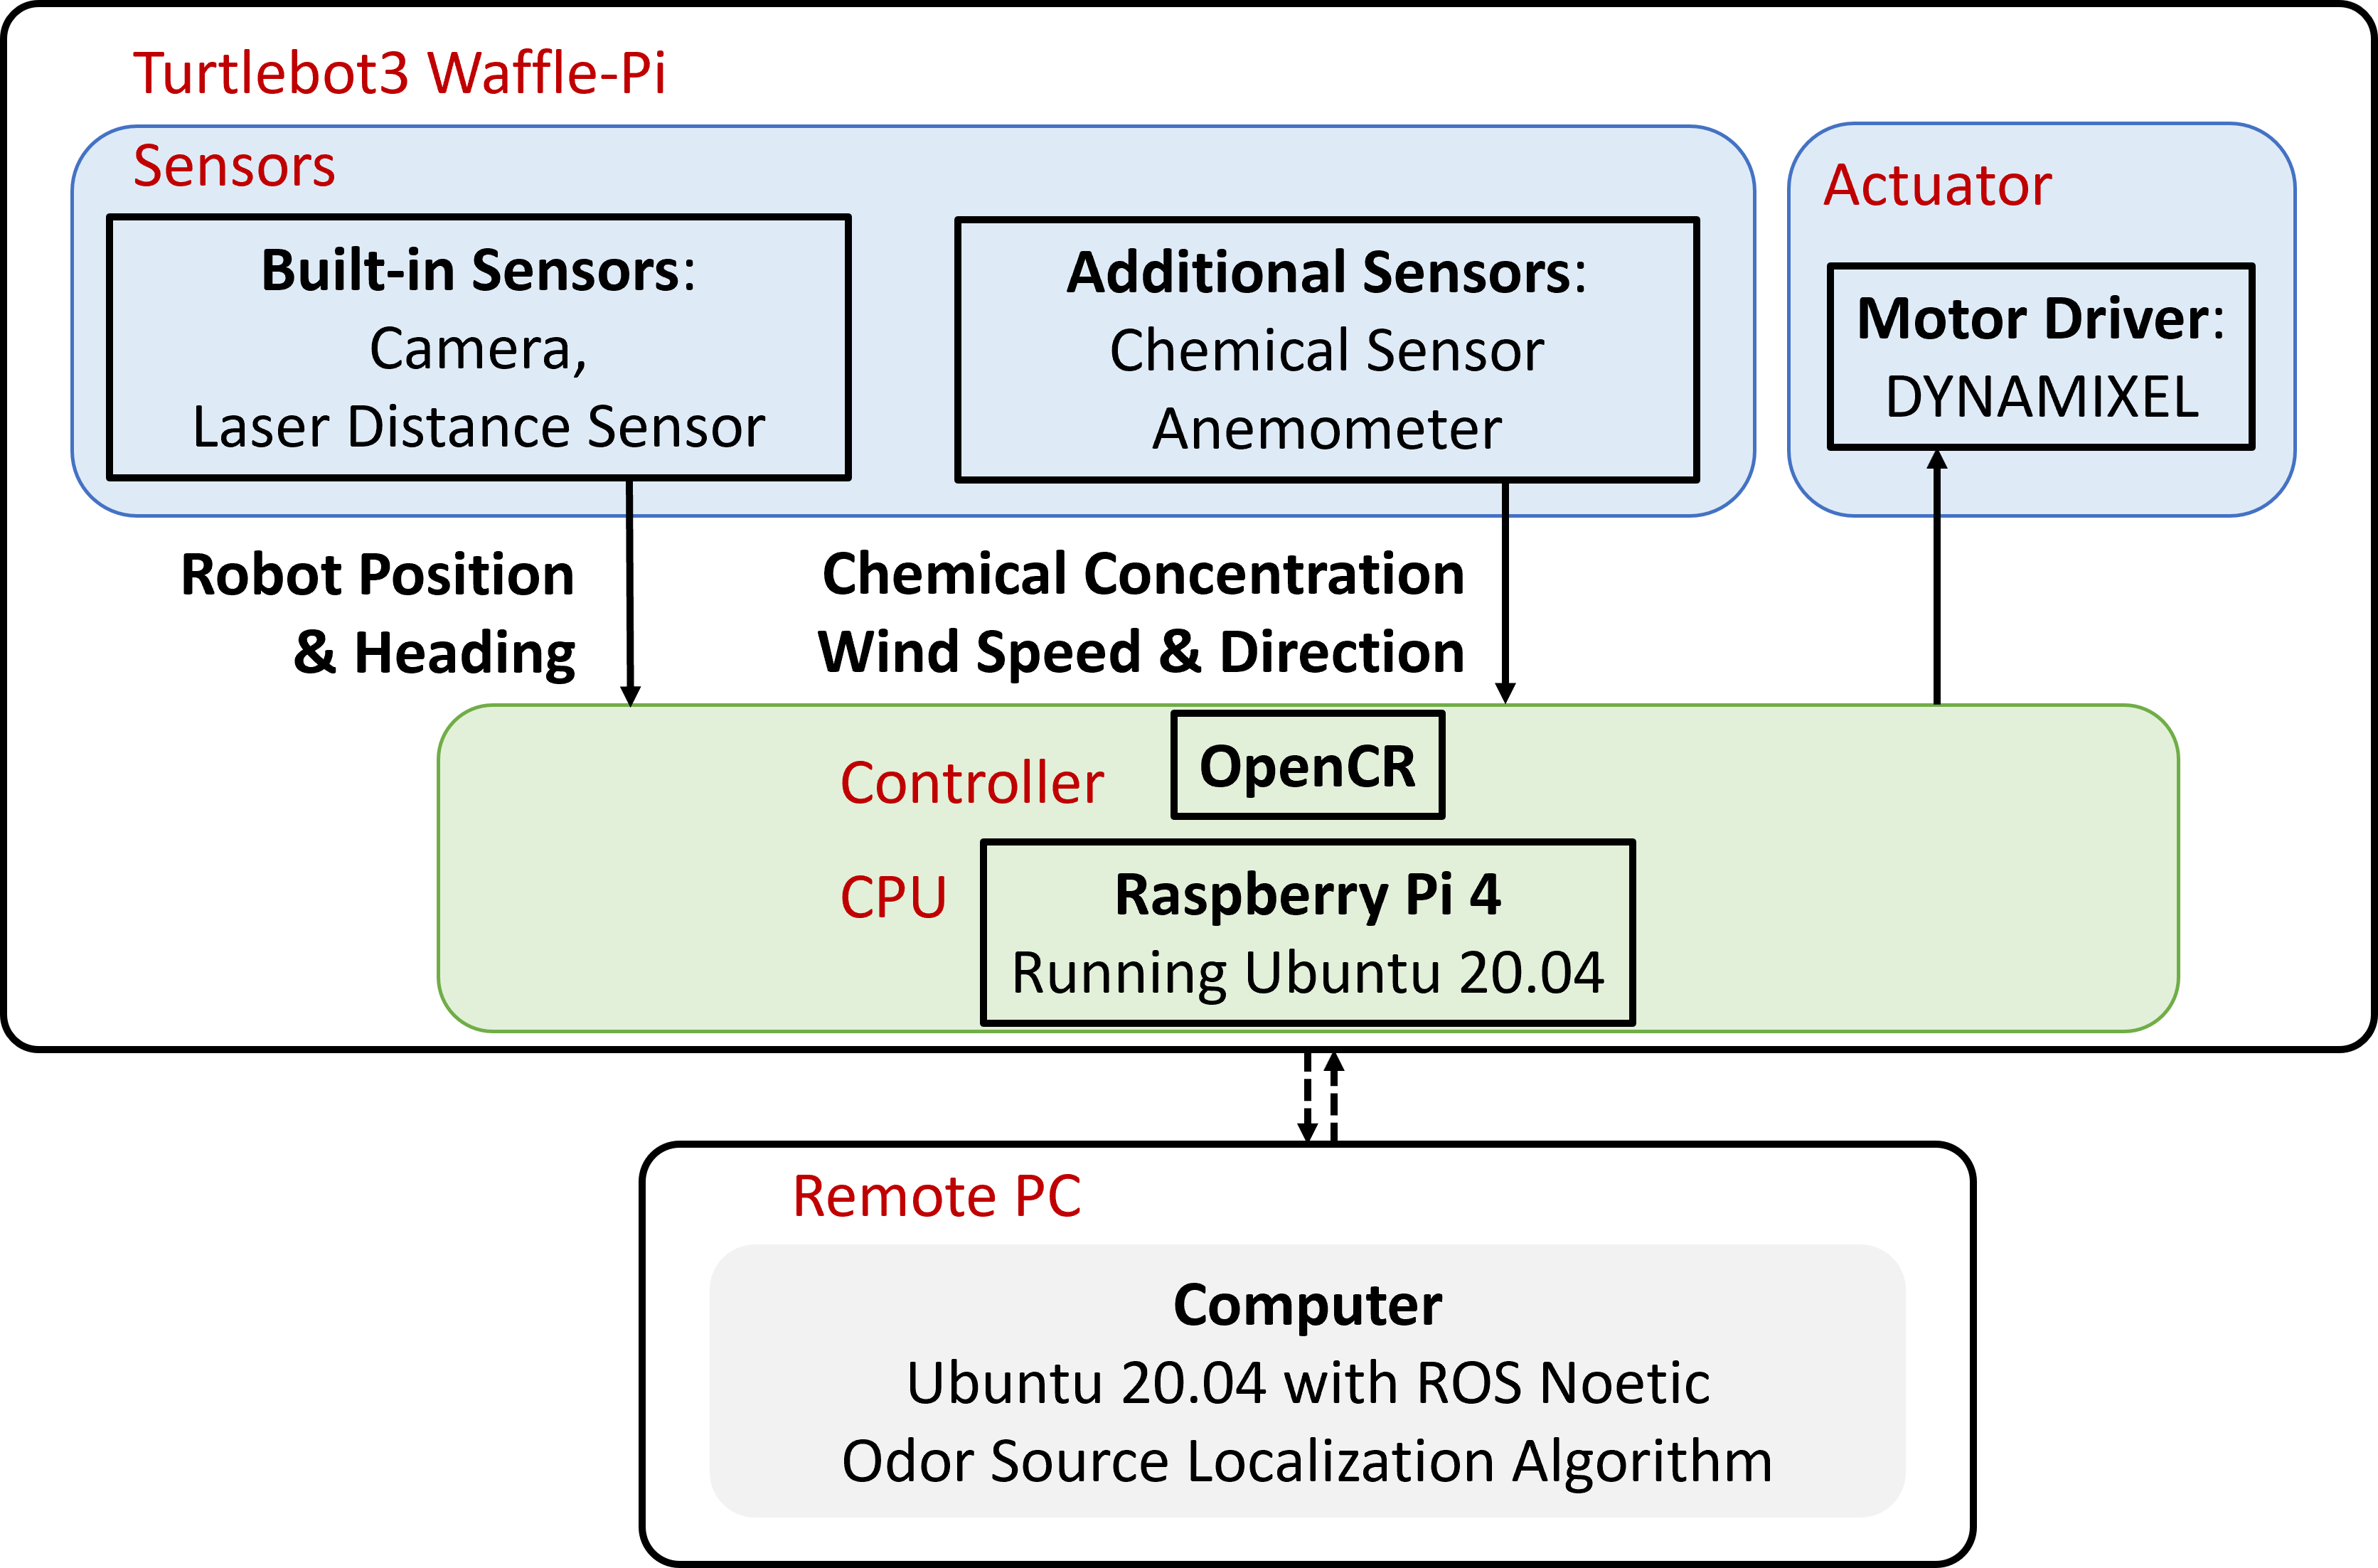
\includegraphics[width=0.9\columnwidth]{Main/Figure/hardware.png}\hspace*{0.04in}
\end{center}
\vspace{-.1in}

\caption
{System configuration. The system consists of two primary components: the Turtlebot3 and a remote PC. The solid line indicates a physical connection, while the dotted line represents a wireless link.}
%\end{singlespace}
\label{fig:OSLhardware}
\end{figure}

The Turtlebot3 features a Raspberry Pi 4 as its CPU, which has limited computing power. It runs on Ubuntu and Robot Operating System (ROS). Ubuntu provides connection capabilities with a remote computer, while ROS allows custom programs on the remote computer to subscribe to specific sensor readings from the robot and publish heading commands back to the robot in real time. ROS supports both Python and C++ programming languages. Figure~\ref{fig:OSLhardware} illustrates the proposed system configuration for the robotic system, which includes a robotic agent (Turtlebot3), an onboard controller, and a ground station (remote Personal Computer or PC). 

For this study, Ubuntu 20.04 and ROS Noetic were installed on both the robot and the remote computer to control the robot. A local area network was used to connect the robot to the remote PC.

Docker is a useful tool for ROS-based robotics research. Different version of the Robot Operating System (ROS) requires different versions of Ubuntu. Docker allows running of Ubuntu from any operating system, including Windows OS. Thus, it allows a consistent and reproducible environment for running robotics research projects.


\subsection{Moth-Inspired ROSL Algorithm}\label{subsec:moth-inspired}
Animals utilize olfaction sensing for locating unknown odor sources \cite{carde2008navigational, nielsen2015olfaction}. Wind sensing is part of animal olfactory behaviors, such as the mate-seeking behaviors of male moths \cite{murlis1992odor}, where a male moth flies against the wind direction to approach the odor source when it detects high odor concentrations. \textcolor{black}{Moth-inspired algorithm is a bio-inspired ROSL algorithm that can lead a mobile robot to an unknown odor source in the environment \cite{shigaki2017time}}.

\begin{figure}[h!]

\ \\
\vspace*{-.18in}

\begin{center}
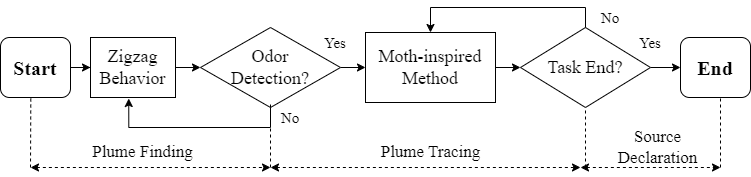
\includegraphics[width=0.7\columnwidth]{Main/Figure/olfaction_flow_diagram.png}\hspace*{0.04in}
\end{center}
\vspace{-.1in}

\caption
{The flow diagram of the proposed ROSL algorithm.}
%\end{singlespace}
\label{fig:mothinspiredFlow_diagram}
\end{figure}

Figure ~\ref{fig:mothinspiredFlow_diagram} presents the flow diagram of the proposed OSL algorithm. An OSL can be divided into three stages, including plume finding, plume tracing, and source declaration \cite{naeem2007chemical}. The first stage of the proposed algorithm is plume finding, which aims to detect plumes in the search area with crosswind 'zigzag' search \cite{wang2022robotic} since the robot has a higher chance to detect odor plumes with crosswind movements than upwind excursions. The robot turns after reaching boundaries and switches to the plume tracing stage after detecting sufficient odor concentration.

In the `Plume Tracing' stage, we proposed a moth-inspired method to command the robot to search for the odor source. The proposed moth-inspired method \cite{farrell2005chemical} can be summarized as the `surge' and `casting' behaviors, as presented in Fig. \ref{fig:olfactionSurgeCasting}. 

\begin{figure}[h]

\ \\
\vspace*{-.18in}

\begin{center}
    \subfigure[`Surge']{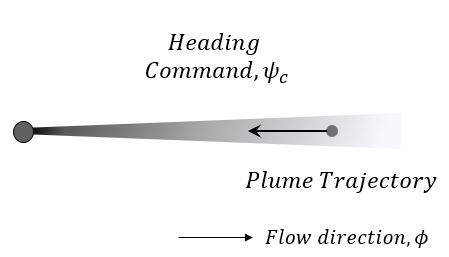
\includegraphics[width=0.4\columnwidth]{Main/Figure/olfaction_surge.png}}\hspace*{0.04in}
    \subfigure[`Casting']{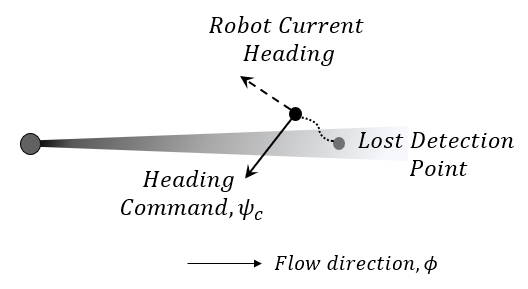
\includegraphics[width=0.4\columnwidth]{Main/Figure/olfaction_casting.png}}\hspace*{0.04in}
\end{center}
\vspace{-.1in}

\caption
{The proposed moth-inspired search behaviors in the `Plume Tracing' stage, including (a) `Surge' behavior and (b) `Casting' behavior.}
%\end{singlespace}
\label{fig:olfactionSurgeCasting}
\end{figure}

\begin{algorithm}[h!]
\caption{`Surge' Behavior}\label{alg:surge}
\begin{algorithmic}[1]
\If{Behavior is `Surge'}
    \State $\psi_{c}=\phi_{Inertial}+180$
    \If{Plume not detected, $D==0$}
        \State \Return `Track-out' Behavior
    \EndIf
\EndIf
\end{algorithmic}
\end{algorithm}

The `surge' behavior is activated when the robot detects odor plumes, i.e., $D=1$. In this behavior, i.e., Algorithm \ref{alg:surge}, the robot moves upwind to progress toward the odor source location. The heading command, i.e., $\psi_c$, in this behavior can be computed via:
\begin{equation}
    \psi_{c}=\phi_{Inertial}+180.
    \label{eqn:surge}
\end{equation}

\begin{algorithm}[h]
\caption{`Casting' Behavior}\label{alg:casting}
\begin{algorithmic}[1]
\If{Behavior is `Casting'}
    \State $\psi_{c}=\phi_{Inertial}+90$
    \If{Plume is detected, $D==1$}
        \State \Return `Surge' Behavior
    \Else
        \State \Return `Casting' Behavior
    \EndIf
\EndIf
\end{algorithmic}
\end{algorithm}

If the robot moves out of plumes, it will activate the 'casting' behavior, i.e., Algorithm \ref{alg:casting}, to move cross-wind until it finds plumes again. During this behavior, the robot uses the equation \ref{eqn:casting} to calculate the target heading $\psi_{c}$.
\begin{equation}
    \psi_{c}=\phi_{Inertial}+90.
    \label{eqn:casting}
\end{equation}
Once the robot re-detects odor plumes, it switches back to the `surge' behavior to continue the upwind movement. These two search behaviors are alternated in the `Plume Tracing' phase until the robot finds the odor source. 

\section{Experiment}\label{Sec:olfactionExperiment}
% ROSL navigation task (search area, navigation to source)
% Performance metric (type/number of tests, analysis and success matric)
\subsection{Navigation Task}\label{Subsec:fusionNavigationTask}

\begin{figure}[h] %% figure

\ \\
\vspace*{-.18in}

\begin{center}
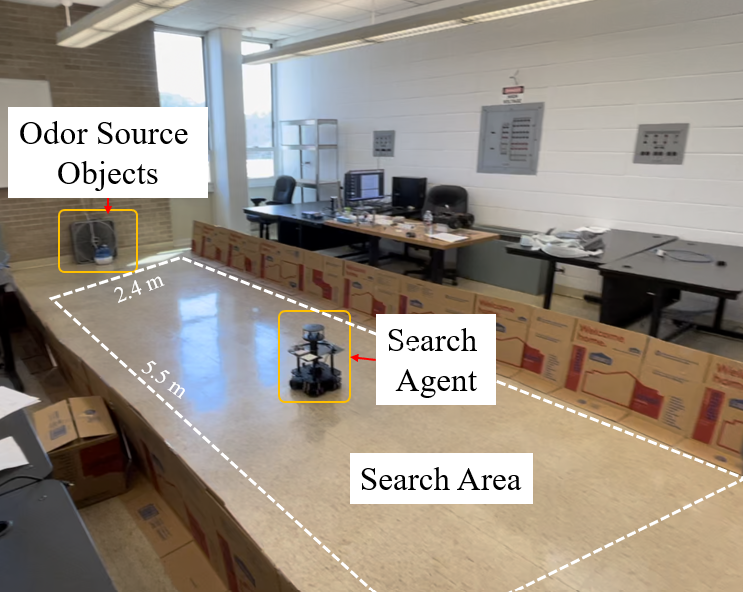
\includegraphics[width=0.9\columnwidth]{Main/Figure/olfaction_SearchArea.png}\hspace*{0.04in}
\end{center}
\vspace{-.1in}

\caption
{The experiment setup. The robot is initially placed at downwind area with the object of finding the odor source. A humidifier loaded with ethanol is employed to generate odor plumes, and an electrical fan is placed behind the humidifier to create an artificial wind field.}
%\end{singlespace}
\label{fig:olfaction_experimentSetup}
\end{figure}

The navigation experiments were conducted in the Automatic Control Lab at the Louisiana Tech University. The lab area was divided into a search area where the robot can navigate and an operation area for the remote PC. In the ROSL experiment, the mobile robot is initiated at a random position in the search area, and it use the sensor data to navigate to the odor source location. The size of the search area is $5.5 m\times2.4m$. A reference map of the search area was created using Simultaneous Localization and Mapping (SLAM). 
Ethanol vapor was used as the odor source as it is not toxic and commonly implemented in OSL research \cite{feng2019experimental}. A humidifier disperses ethanol vapor constantly as the odor plumes. An electric fan was used behind the humidifier to increase odor propagation. The robot was placed away from the odor source in this search area for each trial run. The robot utilized a chemical sensor to read plume concentration and an anemometer to read airflow speed and wind direction. Based on the sensor readings, the moth-inspired algorithm generates robot heading commands until the robot finds the odor source. In this work, the robot is considered as successfully found the odor source if the robot position is within $0.5 m$ of the odor source location.

\section{Results and Discussion}

\begin{figure}[h!] %% figure
\ \\
\vspace*{-.18in}
\begin{center}
    \subfigure{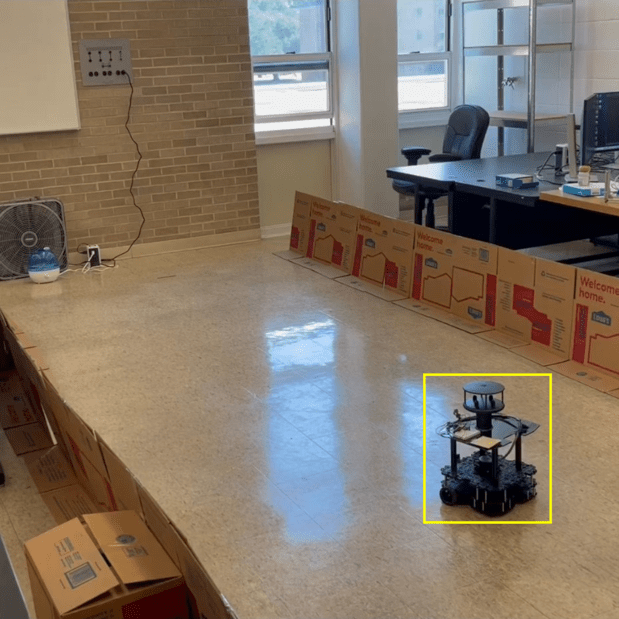
\includegraphics[width=0.33\columnwidth]{Main/Figure/olfaction_t1.png}}\hspace*{0.04in}
    \subfigure{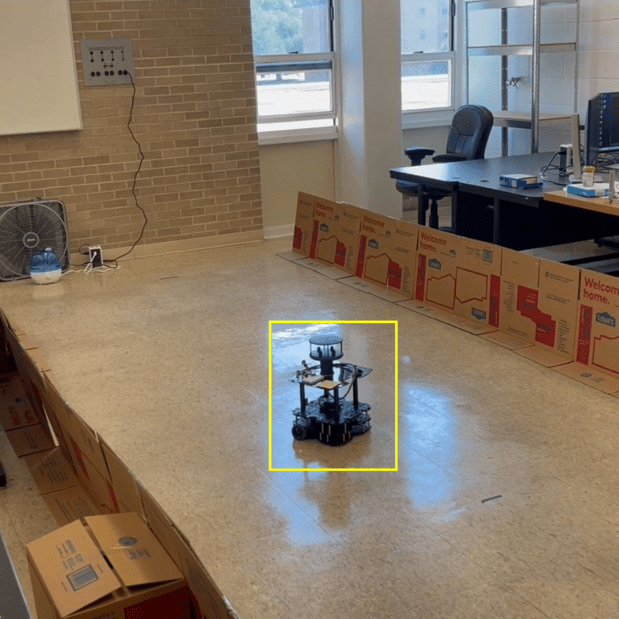
\includegraphics[width=0.33\columnwidth]{Main/Figure/olfaction_t15.png}}\hspace*{0.04in}
    \subfigure{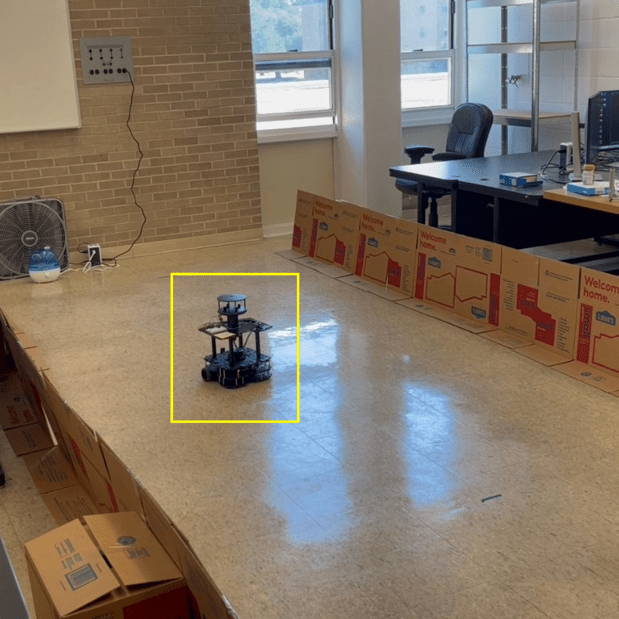
\includegraphics[width=0.33\columnwidth]{Main/Figure/olfaction_t30.png}}\hspace*{0.04in}

    \subfigure{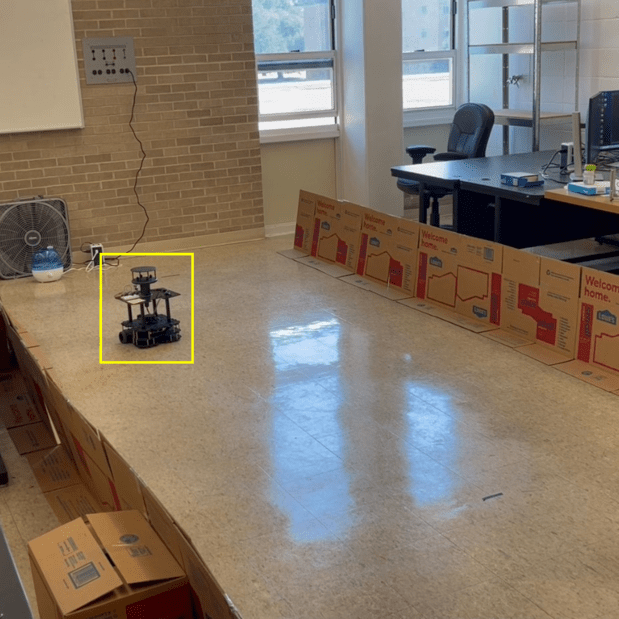
\includegraphics[width=0.33\columnwidth]{Main/Figure/olfaction_t45.png}}\hspace*{0.04in}
    \subfigure{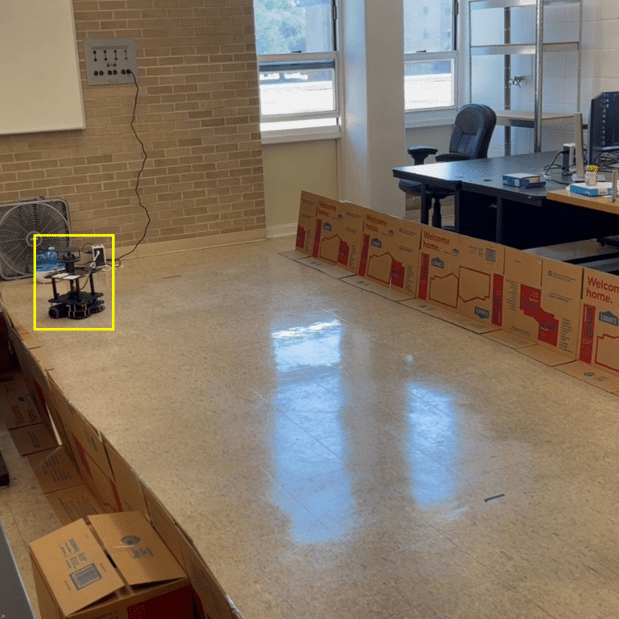
\includegraphics[width=0.33\columnwidth]{Main/Figure/olfaction_t60.png}}\hspace*{0.04in}
    \subfigure{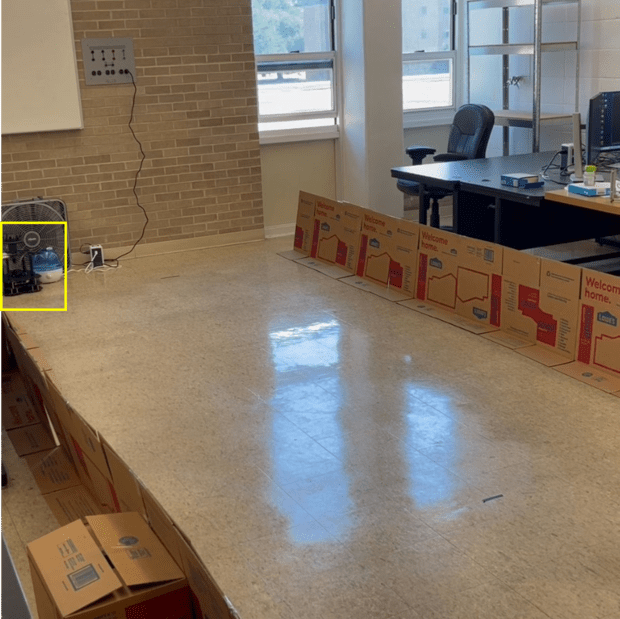
\includegraphics[width=0.33\columnwidth]{Main/Figure/olfaction_t75.png}}\hspace*{0.04in}
\end{center}
\vspace{-.1in}

\caption
{(a) Snapshots of an OSL test with the moth-inspired method. The robot position is highlighted with a yellow rectangle, and the robot correctly finds the odor source at $76$ s.}
%\end{singlespace}
\label{fig:olfaction_snapshots}
\end{figure}


Fig. \ref{fig:olfaction_snapshots} depicts Turtlebot's OSL navigation based on the moth-inspired method. At the start of the search ($t=1$ s), the robot senses odor detection and switches to the 'Plume tracing' stage to trace the odor source location. In this stage, the robot employed the `surge' behavior to move against the wind direction to approach the odor source location (from $t=1$ s to $t=15$ s). Then, the robot lost the plume contact at $t=17$ s and switched to the `casting' behavior to detect plumes in crosswind movements. At $t=30$ s, it reacquired the odor plumes and switched back to the `surge' behavior to move against the wind direction. At $t=45$ s, the robot moves close to the odor source location and remains in the `surge' behavior until it finds the odor source at $t=76$ s. The video of this trial can be found at \footnote{Experiment video link: https://youtu.be/726iJKpz1Ic}.   

The search results of the OSL trials show that the implemented moth-inspired algorithm can successfully navigate a ground mobile robot to the odor source location in a lab environment.